\chapter{课后练习内容和结果}
\label{cp:shell-practice}

本章记录课后实例练习的内容与结果，主要涵盖 Shell 的花括号展开、重定向、引号、退出码、作业控制、别名等基础概念，以及 Vim 编辑器、\verb|time| 计时命令和 Python 调试器 \verb|pdb| 的使用。

\section{第 1 题 花括号展开}

\subsection{实验内容}

如图\ref{fig:brace}所示，使用 \verb|mkdir -p demo/{src,docs,tests}| 命令一次性创建三个目录，然后使用 \verb|ls -F demo| 命令查看创建结果。

\begin{figure}[H]
    \centering
    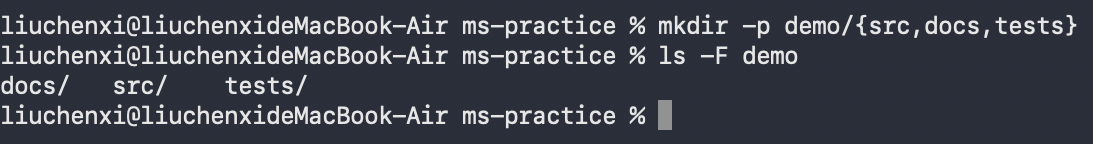
\includegraphics[width=0.8\textwidth]{images2/01_brace.png}
    \caption{花括号展开}
    \label{fig:brace}
\end{figure}

在图\ref{fig:brace}中，\verb|{src,docs,tests}| 是花括号展开（Brace Expansion），Shell 在执行命令前会先把它展开成 \verb|src|、\verb|docs|、\verb|tests| 三个字符串，因此整条命令等价于 \verb|mkdir -p demo/src demo/docs demo/tests|。其中 \verb|-p| 选项表示递归创建目录，父目录不存在时自动创建、已存在时也不报错。\verb|ls| 的 \verb|-F| 选项会在每个条目末尾追加类型标识符，其中 \verb|/| 表示目录。输出 \verb|docs/  src/  tests/| 说明三个目录均已创建成功。

\section{第 2 题 重定向}

\subsection{实验内容}

如图\ref{fig:redirect}所示，先用 \verb|echo "first line" > demo/out.txt| 将第一行内容写入文件，再用 \verb|echo "second line" >> demo/out.txt| 追加第二行内容，最后用 \verb|cat demo/out.txt| 查看文件内容。

\begin{figure}[H]
    \centering
    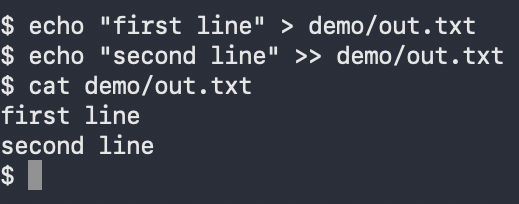
\includegraphics[width=0.7\textwidth]{images2/02_redirect.png}
    \caption{输出重定向与追加重定向}
    \label{fig:redirect}
\end{figure}

在图\ref{fig:redirect}中，\verb|>| 是输出重定向，把命令的标准输出写入指定文件，若文件已存在则先覆盖其内容；\verb|>>| 是追加重定向，把输出追加到文件末尾而不覆盖原有内容。因此第一次写入 first line、第二次追加 second line 之后，out.txt 中依次包含这两行内容。

\section{第 3 题 引号}

\subsection{实验内容}

如图\ref{fig:quotes}所示，先用 \verb|foo=bar| 给变量 \verb|foo| 赋值，然后分别用双引号和单引号打印 \verb|$foo|。

\begin{figure}[H]
    \centering
    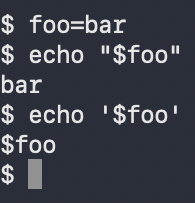
\includegraphics[width=0.35\textwidth]{images2/03_quotes.png}
    \caption{单引号与双引号的区别}
    \label{fig:quotes}
\end{figure}

在图\ref{fig:quotes}中，\verb|echo "$foo"| 使用双引号，其中的变量会发生展开，\verb|$foo| 被替换成变量 \verb|foo| 的值 \verb|bar|，所以输出 \verb|bar|；而 \verb|echo '$foo'| 使用单引号，单引号内的所有字符都按字面量原样处理、不进行变量展开，所以原样输出 \verb|$foo|。

\section{第 4 题 退出码}

\subsection{实验内容}

如图\ref{fig:exitcode}所示，先用 \verb|ls /no_such_dir_xyz| 列出一个不存在的目录（命令失败），再用 \verb|echo $?| 查看上一条命令的退出码；然后执行总是成功的 \verb|true| 命令，再次用 \verb|echo $?| 查看退出码。

\begin{figure}[H]
    \centering
    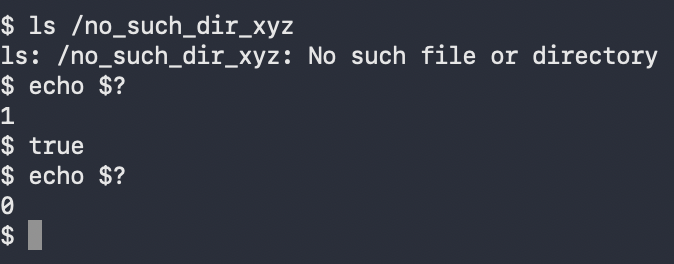
\includegraphics[width=0.7\textwidth]{images2/04_exitcode.png}
    \caption{查看命令的退出码}
    \label{fig:exitcode}
\end{figure}

在图\ref{fig:exitcode}中，\verb|$?| 是 Shell 的内置变量，保存上一条命令的退出码（exit code），其中 0 表示命令执行成功、非 0 表示失败。\verb|ls| 访问不存在的目录时失败，返回退出码 1；而 \verb|true| 是一条不做任何事、总是返回 0 的命令，因此第二次 \verb|echo $?| 输出 0。

\section{第 5 题 作业控制}

\subsection{实验内容}

如图\ref{fig:jobs}所示，依次演示了后台运行、暂停、恢复、终止等 Shell 作业控制操作。

\begin{figure}[H]
    \centering
    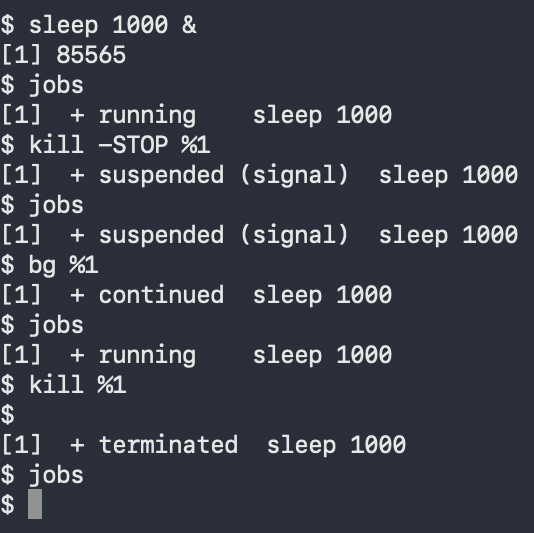
\includegraphics[width=0.55\textwidth]{images2/05_jobs.png}
    \caption{作业控制}
    \label{fig:jobs}
\end{figure}

在图\ref{fig:jobs}中，\verb|sleep 1000 &| 末尾的 \verb|&| 使命令在后台运行，其中 \verb|[1]| 是作业号、\verb|85565| 是该进程的 PID。\verb|jobs| 列出当前 Shell 的所有后台作业，显示作业 1 正在运行（running）。\verb|kill -STOP %1| 向作业 1 发送 SIGSTOP 信号使其暂停（suspended），其中 \verb|%1| 用作业号引用作业。\verb|bg %1| 让暂停的作业在后台继续运行（continued）。最后 \verb|kill %1| 发送默认的 SIGTERM 信号终止作业 1（terminated），此时再执行 \verb|jobs| 列表已为空。

\section{第 6 题 别名}

\subsection{实验内容}

如图\ref{fig:alias}所示，先用 \verb|alias ll="ls -lh"| 定义别名，再用不带参数的 \verb|alias| 查看已定义的别名，最后用 \verb|ll demo| 使用该别名。

\begin{figure}[H]
    \centering
    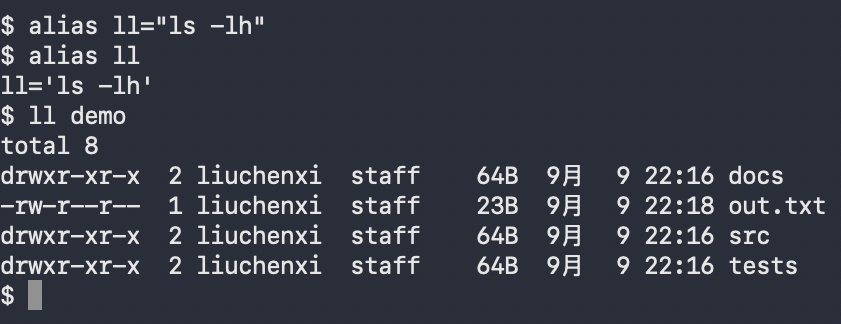
\includegraphics[width=0.75\textwidth]{images2/06_alias.png}
    \caption{定义并使用别名}
    \label{fig:alias}
\end{figure}

在图\ref{fig:alias}中，\verb|alias 名称="命令"| 用于给命令起别名，之后输入别名就等价于输入原命令。\verb|ls -lh| 中 \verb|-l| 表示长格式（显示权限、大小、修改时间等信息），\verb|-h| 表示以人类可读的单位（如 B、KB）显示文件大小。不带参数的 \verb|alias| 会列出当前所有别名，可见 \verb|ll='ls -lh'|。因此执行 \verb|ll demo| 实际就是执行 \verb|ls -lh demo|。

\section{第 7 题 Vim 插入模式}

\subsection{实验内容}

如图\ref{fig:vim_insert}所示，在 Vim 中进入插入模式输入 \verb|print("Hello, Vim!")|；保存退出后，如图\ref{fig:vim_saved}所示用 \verb|cat demo/hello.py| 查看文件内容。

\begin{figure}[H]
    \centering
    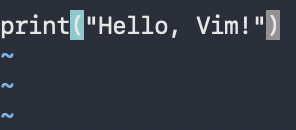
\includegraphics[width=0.4\textwidth]{images2/07a_vim_insert.png}
    \caption{Vim 插入模式}
    \label{fig:vim_insert}
\end{figure}

\begin{figure}[H]
    \centering
    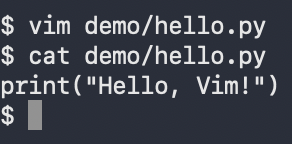
\includegraphics[width=0.4\textwidth]{images2/07b_saved.png}
    \caption{保存并查看文件}
    \label{fig:vim_saved}
\end{figure}

在图\ref{fig:vim_insert}和图\ref{fig:vim_saved}中，使用 \verb|vim demo/hello.py| 打开（或新建）文件 hello.py 后默认处于普通模式，按 \verb|i| 进入插入模式（insert mode），此时可以输入文本 \verb|print("Hello, Vim!")|；输入完成后按 Esc 返回普通模式，再输入 \verb|:wq| 保存并退出。最后用 \verb|cat| 命令查看文件内容，确认写入成功。

\section{第 8 题 Vim 模态编辑}

\subsection{实验内容}

如图\ref{fig:vim_edit}所示，在普通模式下按 \verb|o| 在当前行下方新建一行并进入插入模式，输入第二行 \verb|print("modal editing works")|；保存退出后如图\ref{fig:vim_final}所示文件包含两行内容；最后如图\ref{fig:vim_dw}所示，用 \verb|dw| 命令删除一个单词。

\begin{figure}[H]
    \centering
    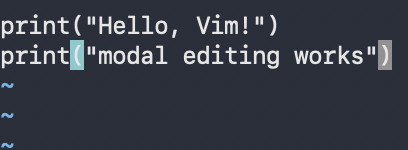
\includegraphics[width=0.5\textwidth]{images2/08a_vim_edit.png}
    \caption{新建一行并输入内容}
    \label{fig:vim_edit}
\end{figure}

\begin{figure}[H]
    \centering
    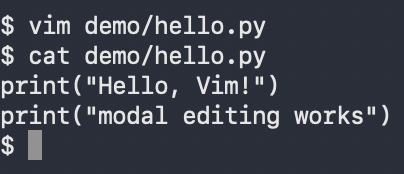
\includegraphics[width=0.5\textwidth]{images2/08b_final.png}
    \caption{保存后的文件内容}
    \label{fig:vim_final}
\end{figure}

\begin{figure}[H]
    \centering
    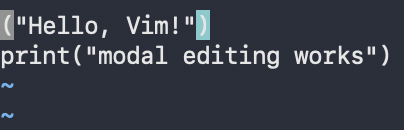
\includegraphics[width=0.5\textwidth]{images2/08c_dw.png}
    \caption{使用 dw 删除单词}
    \label{fig:vim_dw}
\end{figure}

在图\ref{fig:vim_edit}至图\ref{fig:vim_dw}中，Vim 是模态编辑器，普通模式下按键都是命令。\verb|o|（小写 o）在当前行下方另起一行并进入插入模式，用于输入新的一行内容。\verb|dw|（delete word）删除从光标位置到当前单词结尾的内容：把光标移到第一行 \verb|print| 的 \verb|p| 上按 \verb|dw|，即删除 \verb|print| 这一单词，使第一行变为 \verb|("Hello, Vim!")|。

\section{第 9 题 time 计时命令}

\subsection{实验内容}

如图\ref{fig:time}所示，使用 \verb|time| 命令测量 \verb|sleep 1| 的执行时间。

\begin{figure}[H]
    \centering
    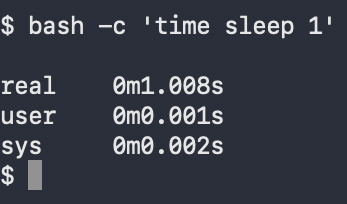
\includegraphics[width=0.5\textwidth]{images2/09_time.png}
    \caption{time 命令计时}
    \label{fig:time}
\end{figure}

在图\ref{fig:time}中，\verb|time 命令| 用于测量命令的执行时间，这里通过 \verb|bash -c 'time sleep 1'| 在 bash 中执行。\verb|sleep 1| 会让进程暂停 1 秒。输出中的 \verb|real| 是命令实际经过的总时间（约 1 秒）；\verb|user| 是用户态 CPU 时间；\verb|sys| 是内核态 CPU 时间。由于 \verb|sleep| 大部分时间处于等待状态，\verb|user| 和 \verb|sys| 都接近 0。

\section{第 10 题 pdb 调试器}

\subsection{实验内容}

如图\ref{fig:pdb}所示，先用 here-document 写入一个 Python 脚本 loop.py，再用 \verb|python3 -m pdb| 调试该脚本。

\begin{figure}[H]
    \centering
    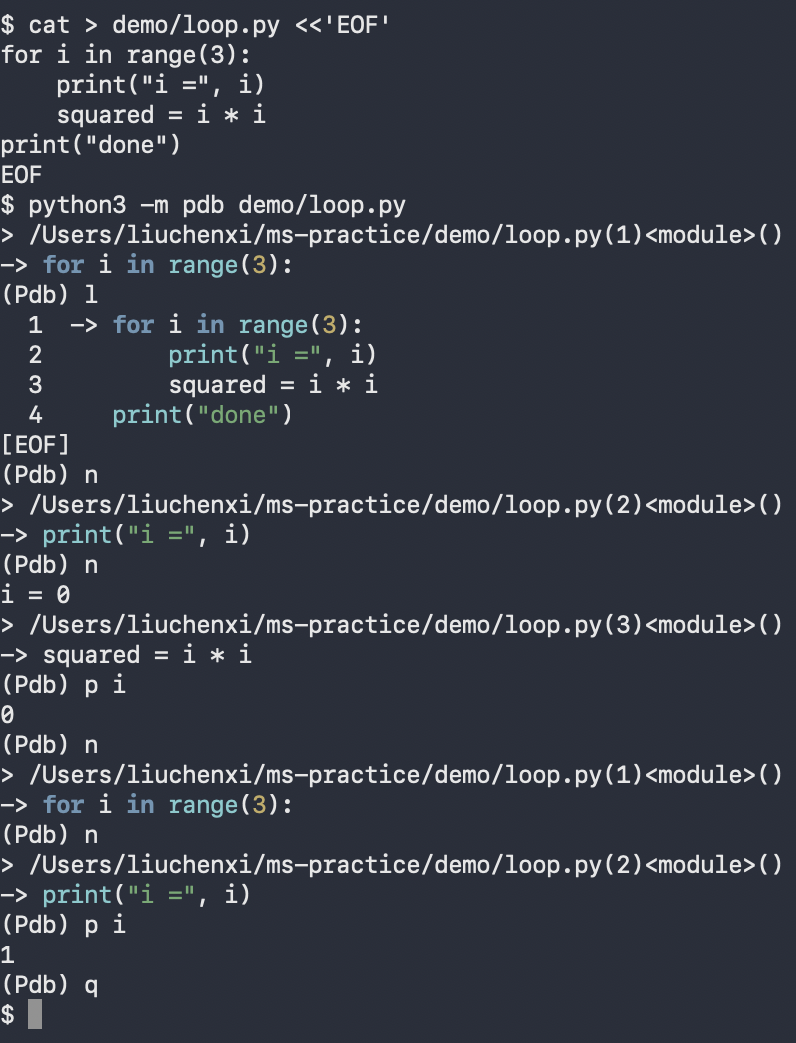
\includegraphics[width=0.6\textwidth]{images2/10_pdb.png}
    \caption{使用 pdb 调试 Python 脚本}
    \label{fig:pdb}
\end{figure}

在图\ref{fig:pdb}中，\verb|cat > demo/loop.py <<'EOF' ... EOF| 是 here-document（此处文档），把 \verb|EOF| 之间的内容原样写入 loop.py 文件，其中 \verb|<<'EOF'| 的单引号表示不对内容做变量展开。写入的脚本为 \verb|for i in range(3)| 的循环，循环体依次打印 \verb|i| 的值并计算 \verb|squared = i * i|，循环结束后打印 \verb|done|。

\verb|python3 -m pdb demo/loop.py| 使用 Python 内置的调试器 pdb 运行脚本，进入交互式调试。其中各调试命令的含义如下：\verb|l|（list）列出当前所在位置的源码；\verb|n|（next）单步执行当前行、不进入函数内部；\verb|p i|（print）打印变量 \verb|i| 的值，图中第一次输出 0、第二次输出 1；\verb|q|（quit）退出调试器。
